\section{TRATAMENTOS AOS DADOS}
\label{sec:tratamentosDados}

Nesta seção são apresentados resumidamente os tratamentos e pré-processamentos realizados sobre os dados da distribuição espaço-temporal dos casos de Influenza no ano de 2009 na cidade de Cascavel/PR, à obtenção de arquivos de entrada utilizados em simulações computacionais. Especificamente, os casos de Influenza são utilizados à obtenção dos arquivos de sazonalidade e distribuição de agentes infectados durante a simulação. As informações obtidas do arquivo de sazonalidade são utilizadas durante a operação de contato entre agentes suscetíveis e infectantes ao controle da taxa de infecção, de acordo com os casos reais observados. O arquivo de distribuição é utilizado à inserção de agentes infectados no ambiente durante a execução de simulações, sendo esses agentes responsáveis pelo início do processo infeccioso da doença. As posições nas quais estes agentes são inseridos correspondem às posições de casos reais de Influenza que foram georreferenciados. 

Aos dados dos $5.089$ casos de Influenza foram realizadas diversas atividades de pré-processamento. Inicialmente foram removidos aproximadamente $155$ casos não georreferenciados ou localizados em regiões não-urbanas da cidade de Cascavel/PR, como zonas rurais e distritos. Em sequência foram mantidos somente os casos com datas de ocorrência entre 17 de Junho e 31 de Dezembro de 2009, pois considerou-se estes casos mais significativos aos propósitos de simulação. Após estas operações restaram $4.658$ casos. Estes casos foram então agrupados por dia de ocorrência dos primeiros sintomas e são empregados à distribuição de agentes infectados durante a execução de simulações e ao cálculos das frações de sazonalidade. A Figura \ref{fig:casos} ilustra a distribuição espacial dos casos de Influenza durante o ano de 2009 e a Figura \ref{fig:casos_acumulados} ilustra o gráfico acumulado dos casos.

\begin{figure}[H]
  \centering
  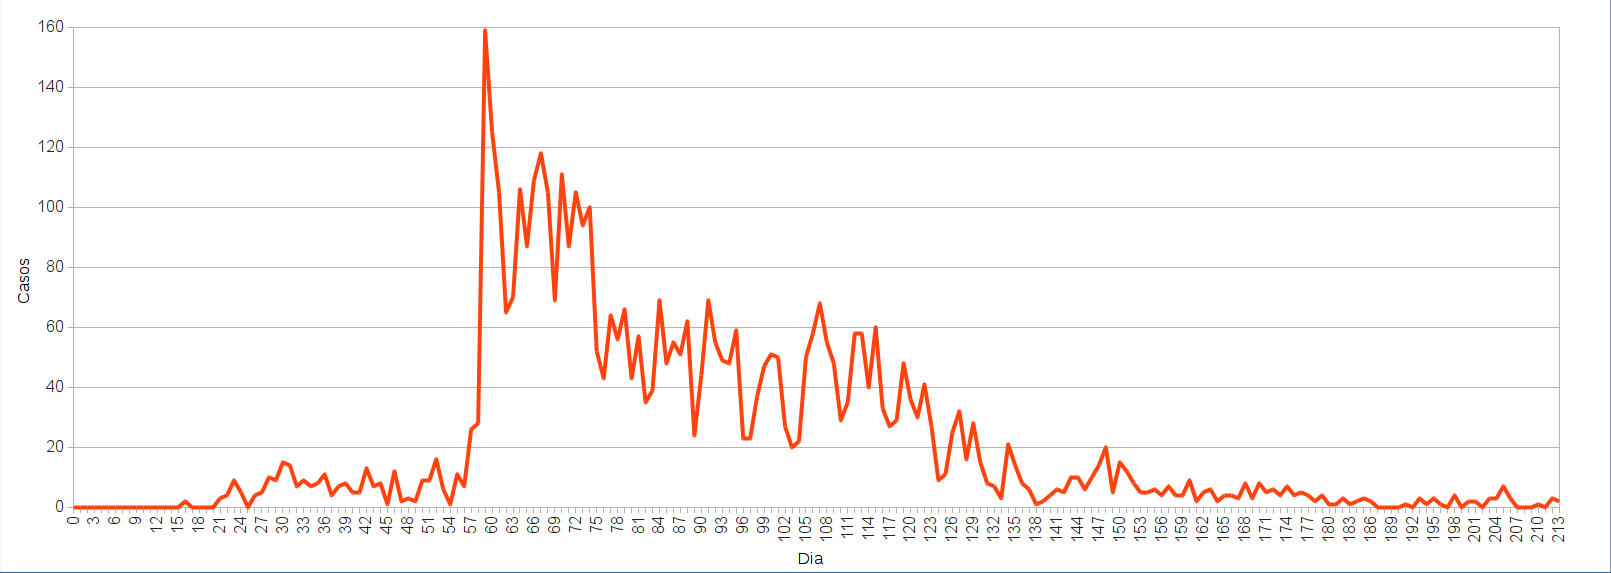
\includegraphics[width=1\textwidth]{Figuras/TratamentosDados/Casos.png}
  \caption{Distribuição temporal dos casos de Influenza}
  \label{fig:casos}
\end{figure} 

\begin{figure}[H]
  \centering
  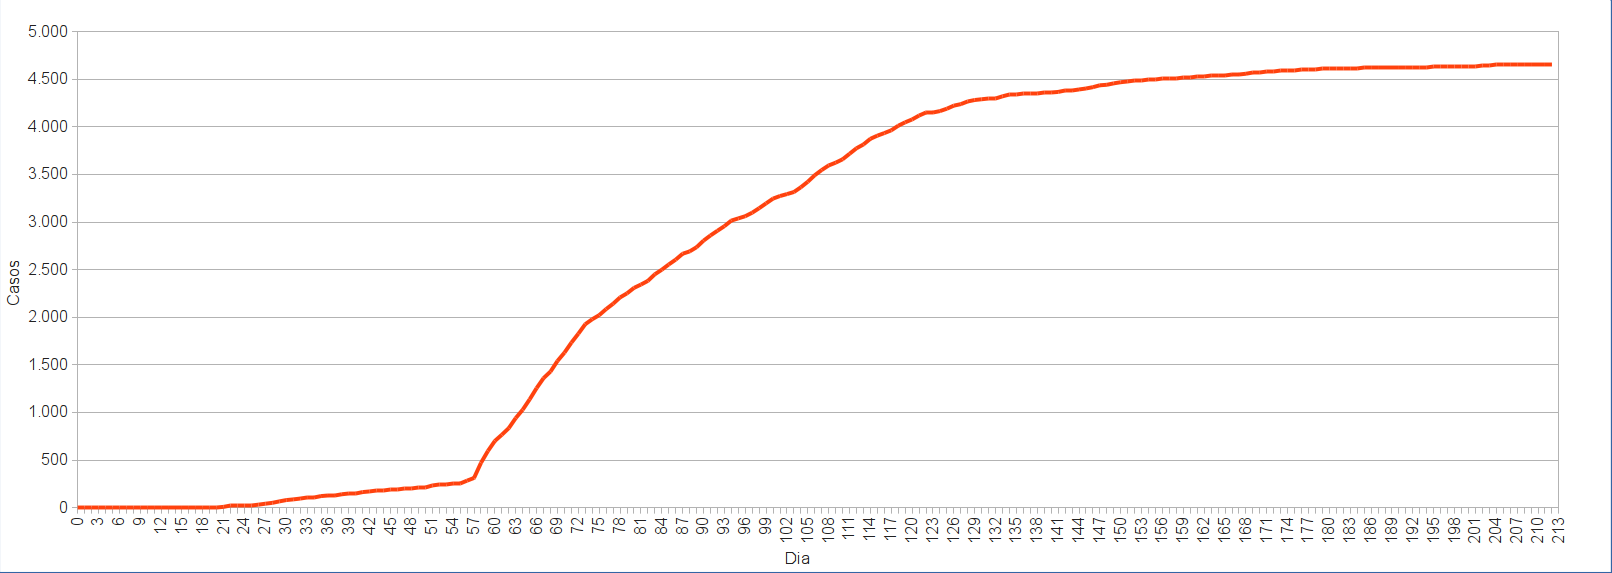
\includegraphics[width=1\textwidth]{Figuras/TratamentosDados/CasosAcumulados.png}
  \caption{Quantidade acumulada dos casos de Influenza}
  \label{fig:casos_acumulados}
\end{figure} 

O percentual de infecção dos agentes suscetíveis em contato com infectados é calculado utilizando-se três distintos parâmetros: os percentuais de infecção adotados às faixas etárias, a fração de sazonalidade do ciclo em que ocorre o contato e uma constante de sazonalidade. Todos esses percentuais são definidos em arquivos de configuração da simulação que são gerados ou manualmente ou por meio do \textit{software} SIMULA. Os percentuais de infecção por faixa etária e a constante de sazonalidade foram definidos de forma empírica por meio de execução de testes. As frações de sazonalidade por ciclo foram definidos com base na distribuição temporal acumulada dos casos de Influenza durante o ano de 2009. A Figura \ref{fig:curva_teorica} ilustra o ajuste realizado aos casos de Influenza utilizando o \textit{software Statistica} e empregando uma função tipo logística acumulada, em que os pontos em azul representam a quantidade normalizada de casos acumulados e em vermelho é ilustrada a curva da equação ajustada. 

\begin{figure}[H]
  \centering
  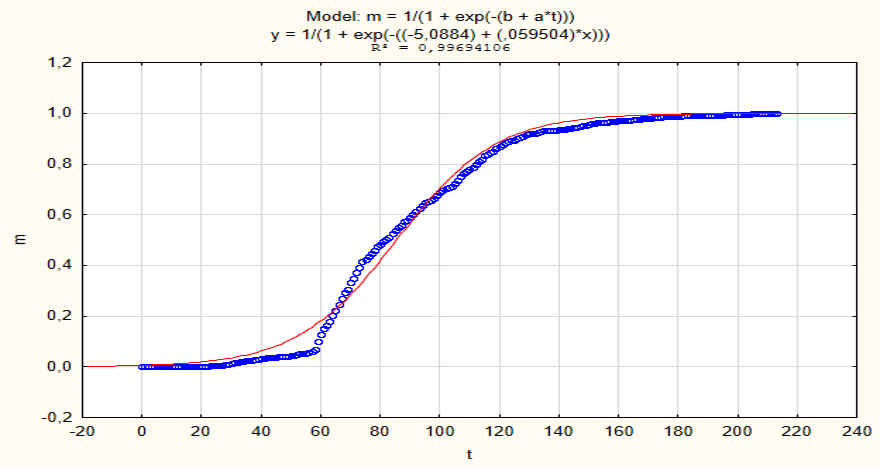
\includegraphics[width=0.8\textwidth]{Figuras/TratamentosDados/Teorico.png}
  \caption{Ajuste aos casos de Influenza utilizando uma função logística acumulada}
  \label{fig:curva_teorica}
\end{figure} 

À definição das frações de sazonalidade foram tomados os complementos das frações apresentadas na Figura \ref{fig:curva_teorica}. Na Figura \ref{fig:percentuais_sazonalidade} é apresentada a curva resultante dos cálculos dos complementos, que são utilizados como frações de sazonalidade durante a simulação à obtenção dos percentuais de infecção de agentes suscetíveis em contato com infectados. 

\begin{figure}[H]
  \centering
  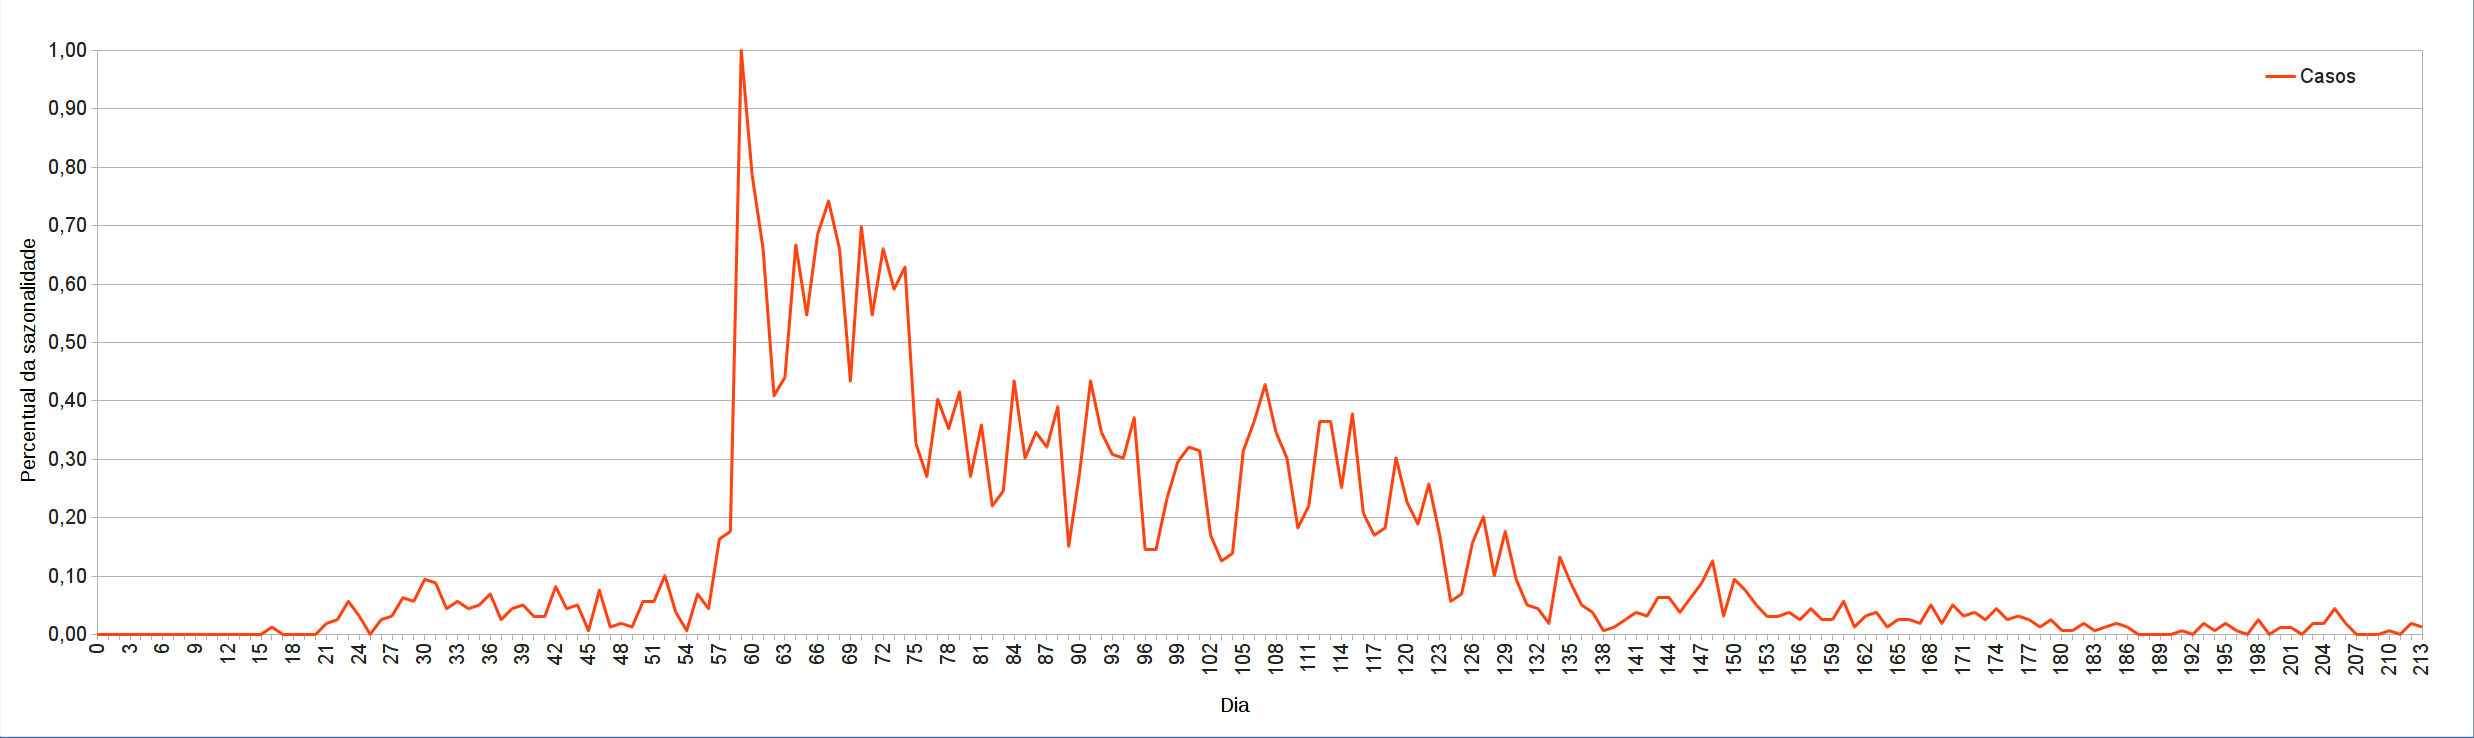
\includegraphics[width=1\textwidth]{Figuras/TratamentosDados/Sazonalidade.png}
  \caption{Distribuição temporal das frações de sazonalidade}
  \label{fig:percentuais_sazonalidade}
\end{figure} 

O arquivo de distribuição de agentes infectados ao longo da simulação é gerado pela função \textit{salvarArquivoDistribuicaoHumanos}, que é ilustrada no Código \ref{cod:salvarArquivoDistribuicaoHumanos}, Algoritmo \ref{alg:salvarArquivoDistribuicaoHumanos} e Figura \ref{fig:salvarArquivoDistribuicaoHumanos}. A função emprega percentuais de casos utilizados e frações de machos e fêmeas para cada faixa etária, de acordo com informações provenientes do banco de dados. Foram utilizadas como base as faixas etárias definidas pelo IBGE, que classificam os indivíduos de acordo com sua idade, como apresentado na Tabela \ref{tab:faixasEtariasIBGE}.  

\begin{table}[H]
\centering
\begin{tabular}{c|c}
 \textbf{Idade} 	& \textbf{Faixa Etária}	\\ \hline
 Menor que 15 anos 	& Criança		\\
 Entre 15 e 24 anos 	& Jovem			\\
 Entre 25 e 59 anos 	& Adulto		\\
 Maior que 59 anos 	& Idosos		\\
\end{tabular}
\caption{Tabela das faixas etárias definidas pelo IBGE.}
\label{tab:faixasEtariasIBGE}
\end{table}

Atualmente, $3\%$ da quantidade total de casos são inseridos durante a execução da simulação. Para as crianças, $51\%$ são masculinos e $49\%$ são femininos. Para os jovens, $50\%$ são masculinos e $50\%$ são femininos. Para os adultos, $48\%$ são masculinos e $52\%$ são femininos. Por fim, para os idosos, $45\%$ são masculinos e $55\%$ são femininos. Na escolha dos casos que serão utilizados inicialmente o conjunto de todos os casos é agrupado por dia de ocorrência. Em seguida, para cada dia são mantidos $3\%$ dos casos. Os casos são então agrupados por faixa etária e os percentuais apresentados anteriormente são utilizados à atribuição aleatória dos sexos. O passo final do algoritmo consiste em atribuir uma posição para a inserção do agente no ambiente, já que os pontos originais dos casos georreferenciados podem não estar presentes no conjunto de pontos interpolados no ambiente. Neste caso, o ponto do ambiente que é mais próximo aquele do caso original é escolhido, considerando-se a distância euclidiana entre eles. 

A Figura \ref{fig:funcoes_logistica} ilustra as curvas obtidas por meio de ajustes realizados aos dados. As quantidades de casos de infecção reais por dia foram normalizados no intervalo $[0.0, 1.0]$ e são ilustrados na cor verde. À esses dados foi ajustada uma equação tipo Logística Acumulada, que é ilustrada na cor vermelha. Na cor azul é ilustrada a equação ajustada aos resultados obtidos por meio de simulação computacional. 

\begin{figure}[H]
  \centering
  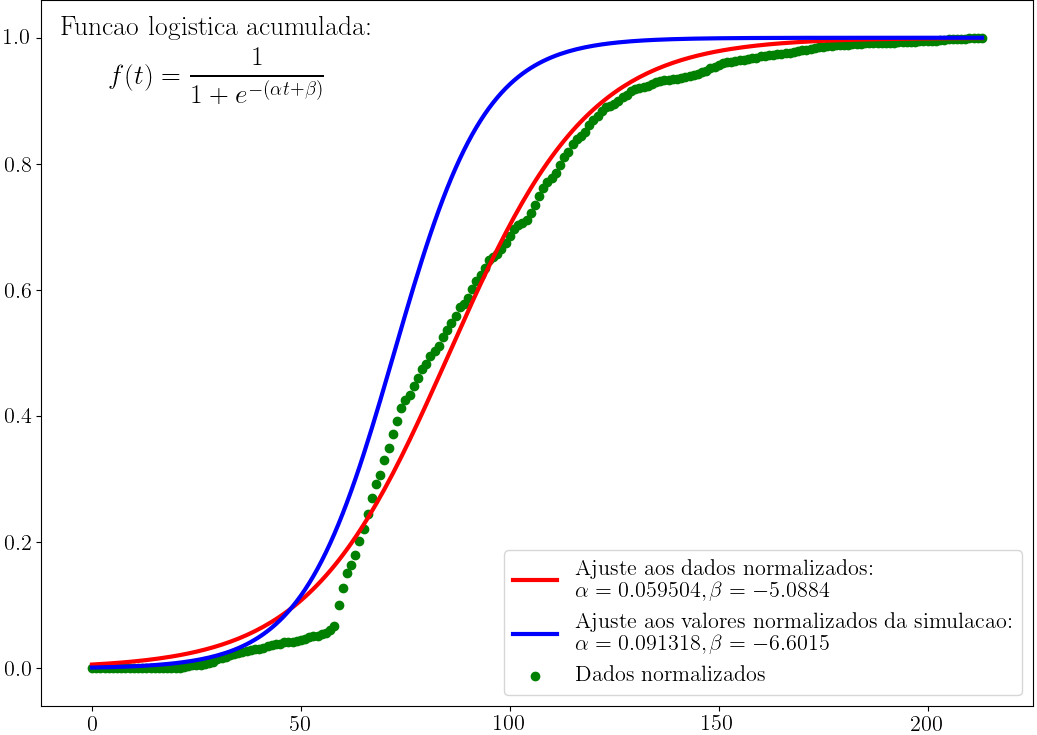
\includegraphics[width=0.7\textwidth]{Figuras/TratamentosDados/Logistica.png}
  \caption{Curvas das equações tipo Logística Acumulada ajustadas aos dados reais e simulados. }
  \label{fig:funcoes_logistica}
\end{figure} 

\newpage